\documentclass[tikz,border=10pt,multi]{standalone}
\usetikzlibrary{positioning,arrows.meta,,bending}
\begin{document}
  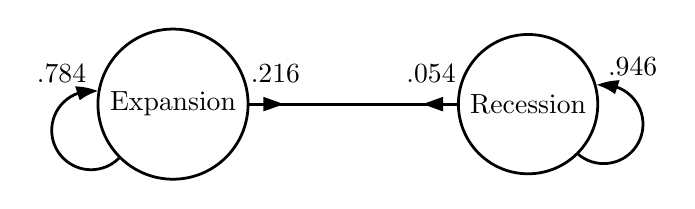
\begin{tikzpicture}
    [
      >/.tip={Triangle[length=7.5pt,width=5pt,bend]},
      line width=1pt,
      my circle/.style={minimum width=10mm, circle, draw},
      my label/.style={above=10pt, anchor=mid}
    ]
    \node (1) [my circle] {Expansion};
    \node (2) [my circle, right=75pt of 1] {Recession};
    \path [postaction={draw, {>[sep=5pt,reversed]}-{<[sep=5pt]}}, draw] (1) -- (2) node [very near start, my label] {$.216$}  node [very near end, my label] {$.054$} ;
    \path [->, draw] (2.south east) arc (-130:100:5mm) node [near end, my label] {$.946$};
    \path [->, draw] (1.south west) arc (-45:-280:5mm) node [near end, my label] {$.784$};
  \end{tikzpicture}
\end{document}
